\documentclass{beamer}
\usepackage{Res/tex/presento}

\usepackage{amsfonts, amssymb, amsmath, amsthm, enumerate}
\usepackage{xcolor, graphicx, tikz}
\usepackage{multicol}

\newcommand{\Nat}{\ensuremath \mathbb{N}}
\newcommand{\Int}{\ensuremath \mathbb{Z}}
\newcommand{\Rat}{\ensuremath \mathbb{Q}}
\newcommand{\Real}{\ensuremath \mathbb{R}}
\newtheorem*{teo}{Teorema}
\newtheorem*{df}{Definicija}
\newenvironment{thinker}{\begin{alertblock}{Zavrzlama}}{\end{alertblock}}
\newenvironment{construct}{\begin{block}{Skalamerija}}{\end{block}}
\newenvironment{idea}{\begin{block}{Ideja}}{\end{block}}
\newenvironment{sidenote}{\begin{alertblock}{Inače}}{\end{alertblock}}
\newcommand{\Background}[2]{
    \tikz[remember picture, overlay] \node[opacity=#2, at=(current page.center)] {
        \includegraphics[height=\paperheight]{#1}
    };
}

\begin{document}
    {
\usebackgroundtemplate{%
\tikz[overlay,remember picture] \node[opacity=0.5, at=(current page.center)] {
  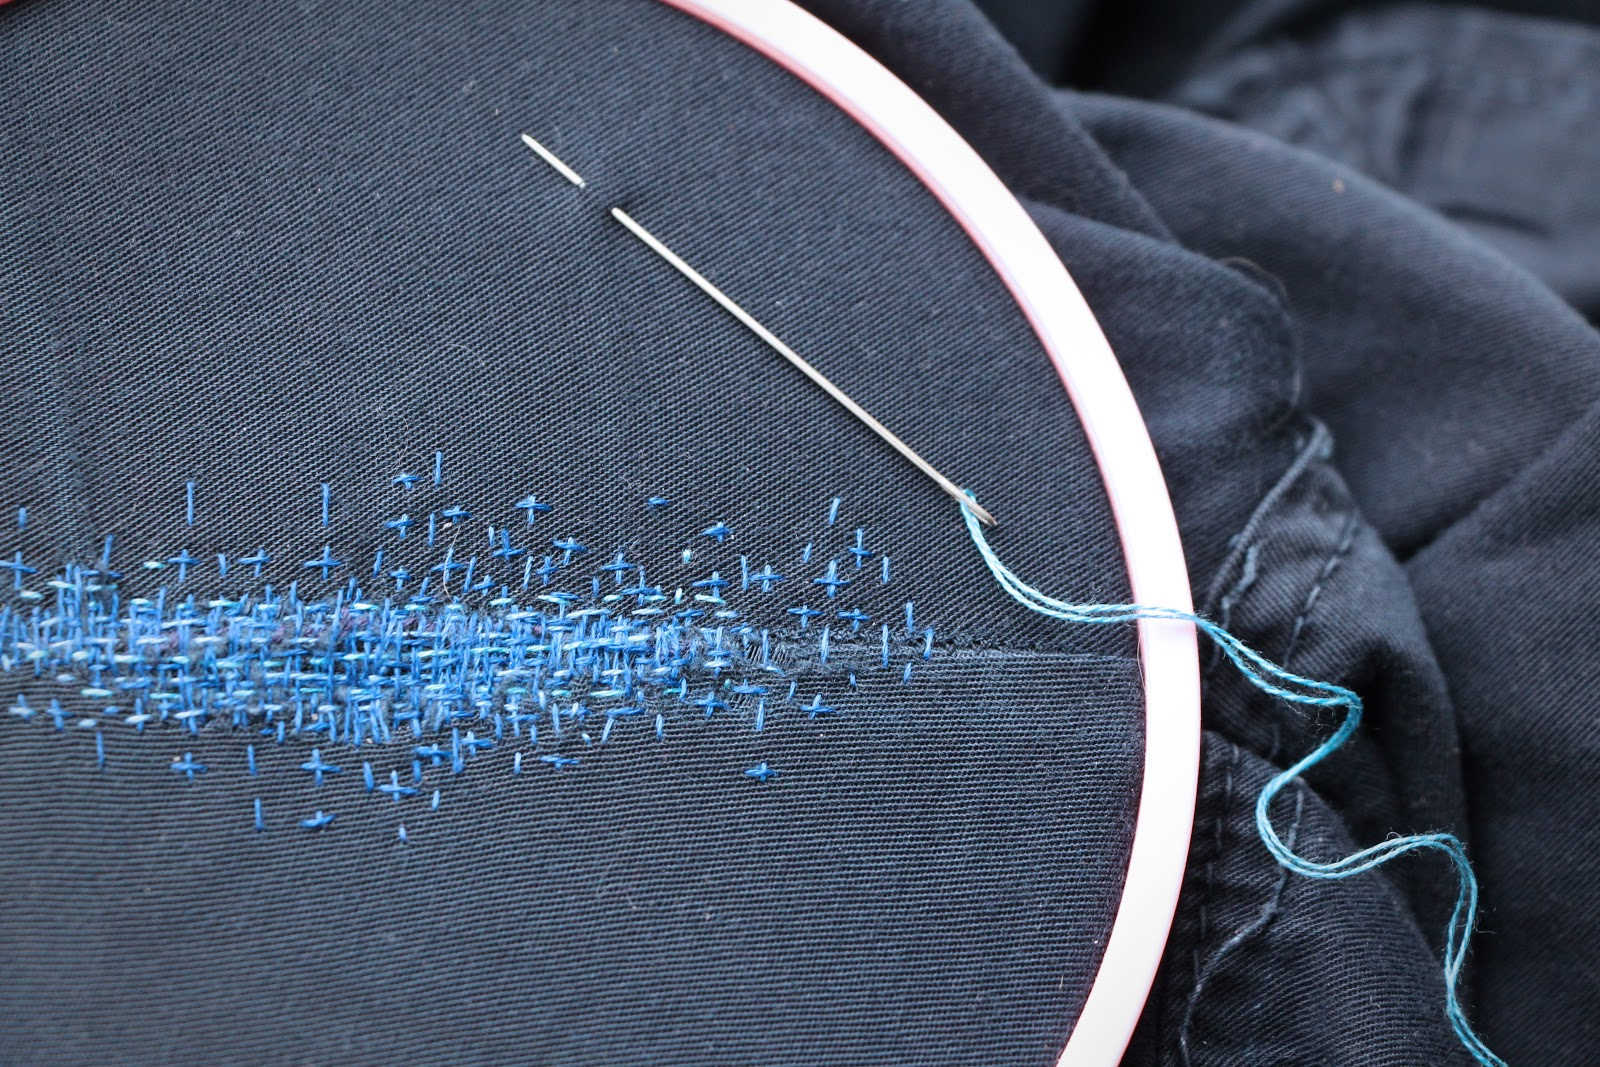
\includegraphics[height=\paperheight]{Res/img/krpljenje}};
}
\begin{frame}[plain]
    \vfill
    \largetext{
        \color{orange}{Dimitrije Glukčević  \\
        \setnote{dimchee90@gmail.com}}
    }
    \scalebox{0.5}{\input{Res/img/pmf.pdf_tex}}
    \vfill
    \largetext{\color{colorblue}
        O raznizavanju i krpljenju
    } \\
    \setnote{Zimski seminar za mlađe polaznike, Petnica 2022}
\end{frame}
}

    \begin{framebg}{Lakiranje rama}{Res/img/coating}{0.5}
    \end{framebg}
    \framecard{\Huge{Lakiranje kocke?}}

    \begin{framebg}{}{Res/img/operation}{0.5}
    \end{framebg}
    \begin{framebg}{Grupe}{Res/img/group}{0.5}
        \begin{enumerate}
            \itemR $(a \circ b) \circ c = a \circ (b \circ c)$
            \itemR $\exists e \forall a \quad a \circ e = e \circ a = a$
            \itemR $\forall a \exists a^{-1}  \quad a \circ a^{-1} = a^{-1} \circ a = e$
            \item[${\color{magenta} \rightarrow}$] $a \oplus b = b \oplus a$
        \end{enumerate}
    \end{framebg}
    \framecard{\Huge{Na koliko načina možemo da rotiramo kocku?}}
    \begin{framebg}{Izomorfizmi}{Res/img/reflection}{0.7}
        \begin{df}[Permutacija]
            Permutacija je bilo koja bijekcija skupa u samog sebe.
        \end{df}
        \begin{teo}[Kejli]
            Svaka grupa je izomorfna nekoj grupi permutacija
        \end{teo}
    \end{framebg}
    \begin{framebg}{Kocka je bačena (jer je loše izlakirana)}{Res/img/rubic}{0.5}
        $$S_4 \cong \langle s_1, s_2, s_3 \mid 
            s_1^2 = s_2^2 = s_3^2 = (s_1s_2)^2 = (s_2s_3)^3 = (s_1s_3)^3 = e \rangle
        $$
        \begin{idea}
            Svaki dan farbamo 3, a ne 1 stranu!
        \end{idea}
    \end{framebg}
    \begin{framebg}{Geometrijska začkoljica}{Res/img/geometry}{0.7}
        \begin{thinker}
            Kako predstaviti kretanje po prostoru?
        \end{thinker}
        %\pause
        \begin{thinker}
            Šta su vektori?
        \end{thinker}
    \end{framebg}
    \begin{framebg}{Prostranstva}{Res/img/trait}{0.4}
        $u, v \in V \qquad \alpha, \beta \in \mathbb{K}$
        \begin{multicols}{2}
            \begin{itemize}
                \itemR  $1 \circ u = u$
                \itemR  $\alpha \circ (u \oplus v) = \alpha \circ u \oplus \alpha \circ v$
                \itemR  $(\alpha \oplus \beta) \circ u = \alpha \circ u \oplus \beta \circ u$
                \itemR  $\alpha \circ (\beta \circ u) = (\alpha \cdot \beta) \circ u$
            \end{itemize}
            \columnbreak
            \begin{itemize}
                \item[$\color{magenta} \rightarrow$] $0 \vec u = \vec 0$
                \item[$\color{magenta} \rightarrow$] $\alpha \vec 0 = \vec 0$
                \item[$\color{magenta} \rightarrow$] $\alpha \vec u = \vec 0 \implies \alpha = 0 \lor \vec u = \vec 0$
                \item[$\color{magenta} \rightarrow$] $(-1)  \vec u = \underbar {\vec u}$
                \item[$\color{magenta} \rightarrow$] $(-\alpha) \vec u = \underbar {\alpha \vec u}$
            \end{itemize}
        \end{multicols}
    \end{framebg}
    \begin{framebg}{Kombinacije}{Res/img/span}{0.5}
        \begin{itemize}
            \itemR $\mathcal L(M) = \{ v \in V \mid v \text{ je linearna kombinacija vektora iz } M \}$
            \itemR $dim V = |B|, \text{ gde je B neki bazni skup }$
            \itemR $V \cong \mathbb{K}^{dim V}$
        \end{itemize}
    \end{framebg}
    \framecard{\Huge{Zašto je $\Real^3$ trodimenzionalan?}}
    \begin{framebg}{Ponizni vektori}{Res/img/fibonacci}{0.4}
        {$\color{blue} \rightarrow$} Nizovi gde je svaki sledeći član
        jednak zbiru prethodna 2 čini vektorski prostor!
        \begin{thinker}
            Koliko dimenzionalan je ovaj prostor?
        \end{thinker}
    \end{framebg}
    \begin{framebg}{Zvuk slike}{Res/img/ATD}{0.9}
    \end{framebg}
    \begin{framebg}{Perspektiva}{Res/img/speakers}{0.5}
        $\text{Zvučnik} \cong A(t) \cdot p(x, y, z, t)$
        \begin{idea}
            Funkcije su vektori!
        \end{idea}
    \end{framebg}
    \begin{frame}{3Blue1Brown}
        \tikz[remember picture, overlay] \node[at=(current page.center)] {
            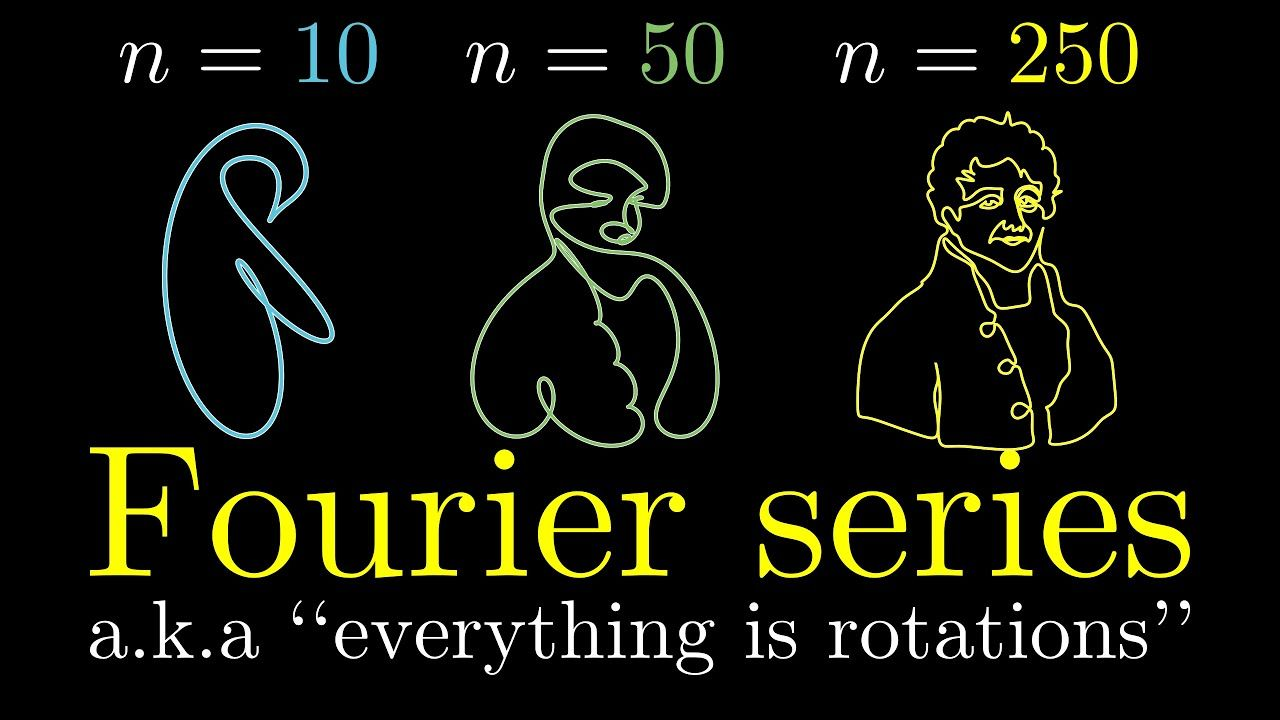
\includegraphics[width=0.8\paperwidth]{Res/img/fourier}
        };
    \end{frame}
    \begin{framebg}{Linearna preslikavanja}{Res/img/mapping}{0.5}
        \begin{df}
            Preslikavanje $f : \mathbb V \to \mathbb W$ je linearno ako važi:
            $$f(\alpha \vec x + \beta \vec y) = \alpha f(\vec x) + \beta f(\vec y)$$
        \end{df}
        \begin{thinker}
            Izračunati $f(\vec 0_{\mathbb V})$
        \end{thinker}
    \end{framebg}
    \begin{framebg}{Red or Blue}{Res/img/morpheus}{0.7}
        \begin{teo}
            Prostor svih linearnih preslikavanja $f : \mathbb V \to \mathbb W$ u oznaci
            $Hom(\mathbb V, \mathbb W)$ je vektorski
            prostor dimenzije $dim \mathbb V \cdot dim \mathbb W$
        \end{teo}
        \begin{df}[Dualan prostor]
            Prostor funkcija $Hom(\mathbb V, \mathbb K)$ je dimenzije $dim \mathbb V$,
            pa je sa njim izomorfan. Elementi ovog prostora nazivaju se \textbf{linearne funkcionele}.
        \end{df}
    \end{framebg}
    \begin{framebg}{Igrice}{Res/img/game}{0.5}
        \begin{align*}
            \begin{pmatrix}
                x & 0 & 0 & 0 \\
                0 & y & 0 & 0 \\
                0 & 0 & z & 0 \\
                0 & 0 & 0 & 1
            \end{pmatrix} &
            \begin{pmatrix}
                \frac{2n}{r-l} & 0 & \frac{r+l}{r-l} & 0 \\
                0 & \frac{2n}{t-b} & \frac{t+b}{t-b} & 0 \\
                0 & 0 & \frac{f+n}{f-n} & \frac{2nf}{f-n} \\
                0 & 0 & -1 & 0
            \end{pmatrix} \\
            \begin{pmatrix}
                1 & 0 & 0 & x \\
                0 & 1 & 0 & y \\
                0 & 0 & 1 & z \\
                0 & 0 & 0 & 1
            \end{pmatrix} &
            \begin{pmatrix}
                cos \theta & -sin \theta & 0 & 0 \\
                sin \theta &  cos \theta & 0 & 1 \\
                0 & 0 & 1 & 0 \\
                0 & 0 & 0 & 1
            \end{pmatrix}
        \end{align*}
    \end{framebg}
    \begin{frame}{Kvadratići}
        %\pause
        \begin{thinker}
            Šta su ovde vektori? Kako se sabiraju, a kako skaliraju i čime?
        \end{thinker}
        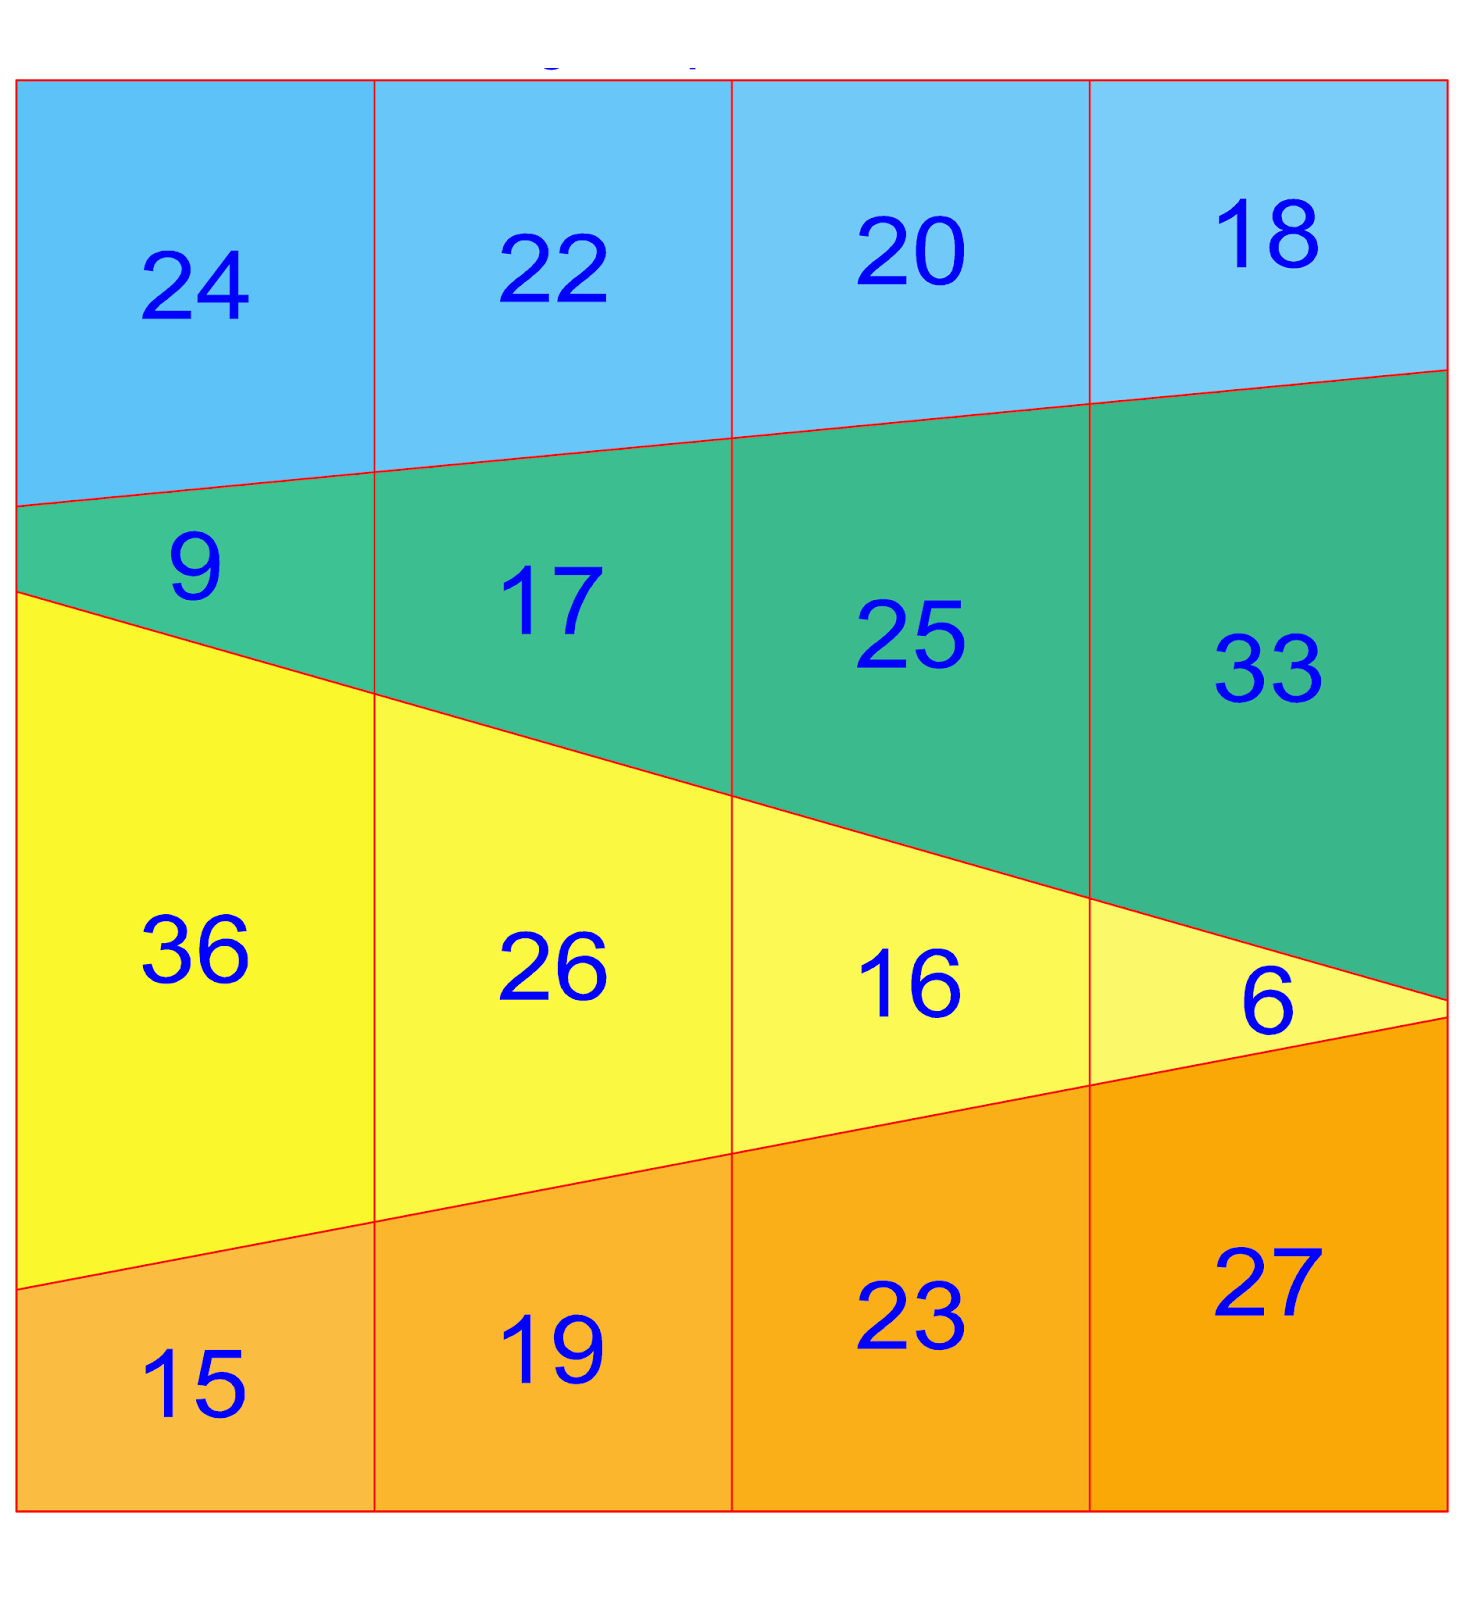
\includegraphics[height=\textheight]{Res/img/magic_square}
    \end{frame}
    \begin{frame}{Baza}
    \tiny
    \begin{align*}
        \begin{pmatrix}
            1&1&1&1\\
            1&1&1&1\\
            1&1&1&1\\
            1&1&1&1
        \end{pmatrix} &
        \begin{pmatrix}
            1&0&0&-1\\
            0&-1&1&0\\
            0&1&-1&0\\
            -1&0&0&1
        \end{pmatrix} &
        \begin{pmatrix}
            1&-1&0&0\\
            -1&1&0&0\\
            0&0&-1&1\\
            0&0&1&-1
        \end{pmatrix} &
        \begin{pmatrix}
            0&0&0&0\\
            1&0&0&-1\\
            -1&0&0&1\\
            0&0&0&0
        \end{pmatrix} \\
        \begin{pmatrix}
            1&0&-1&0\\
            0&-1&0&1\\
            -1&0&1&0\\
            0&1&0&-1
        \end{pmatrix} &
        \begin{pmatrix}
            0&0&-1&1\\
            0&0&1&-1\\
            1&-1&0&0\\
            -1&1&0&0
        \end{pmatrix} &
        \begin{pmatrix}
            0&-1&0&1\\
            1&0&-1&0\\
            0&1&0&-1\\
            -1&0&1&0
        \end{pmatrix} &
        \begin{pmatrix}
            0&1&-1&0\\
            0&0&0&0\\
            0&0&0&0\\
            0&-1&1&0
        \end{pmatrix}
    \end{align*}
\end{frame}

    \framecard{
        Mnogo ljudi došlo je na svadbu, zapravo ispostavilo se da su došli svi,
        odnosno na kraju nije više bilo mesta za sedenje. Međutim, niko nije bio obavešten o
        rasporedu sedenja. Koja je verovatnoća da niko nije seo na predviđeno mesto?
    }
    \begin{framebg}{}{Res/img/inclusion}{0.5}
        $$ \left| \binom{\{A_1,...,A_n\}} k \right| = \binom n k = \frac {n!} {k! (n-k)!}
        $$
        $$(a + b)^n = \sum_{k=0}^n \binom n k a^k b^{n-k}
        $$
        $$\left| \bigcup_{i=1}^n A_i\right| = 
         \sum_{k=1}^n (-1)^{k+1}\sum_{F \in \binom{\{A_1,...,A_n\}} k} \left| \bigcap F \right|
        $$

    \end{framebg}
    \begin{framebg}{Svadba}{Res/img/wedding}{0.5}
        \pause
        \begin{itemize}
            \itemR Za $n=2$  je $P = 0$ \pause
            \itemR Za $n=2$  je $P = 0.5$ \pause
            \itemR Za $n=3$  je $P \approx 0.333333$ \pause
            \itemR Za $n=4$  je $P = 0.375$ \pause
            \itemR Za $n=5$  je $P \approx 0.366667$ \pause
            \itemR Za $n=7$  je $P \approx 0.367857$ \pause
            \itemR Za $n=10$ je $P \approx 0.367879$ \pause
            \itemR Za $n \to \infty$ je $P \approx 1/e$
        \end{itemize}
    \end{framebg}
    \framecard{\Huge Hvala na pažnji!}
\end{document}
